% $Header: /cvsroot/latex-beamer/latex-beamer/solutions/generic-talks/generic-ornate-15min-45min.en.tex,v 1.5 2007/01/28 20:48:23 tantau Exp $

\documentclass{beamer}

\mode<presentation>
{
  \usetheme{Singapore}
  % or ...

  \setbeamercovered{transparent}
  % or whatever (possibly just delete it)
}


\usepackage[brazil]{babel}
\usepackage[utf8]{inputenc}
\usepackage{times}
\usepackage[T1]{fontenc}
\usepackage{graphicx}
\usepackage{amssymb}
\usepackage{epstopdf}



\title[Plataforma para Estudo Interativo de Métodos Econométricos] % (optional, use only with long paper titles)
{Uma Plataforma de Software para o Estudo Interativo de Métodos e Algoritmos Econométricos}

%\subtitle
%{Presentation Subtitle} % (optional)

\author % (optional, use only with lots of authors)
{Carlos Duarte do Nascimento}
% - Use the \inst{?} command only if the authors have different
%   affiliation.


\institute[Universidade de São Paulo] % (optional, but mostly needed)
{
  Instituto de Matemática e Estatística\\
  Universidade de São Paulo
%  \and
%  \inst{2}%
%  Faculdade de Economia, Administração e Contabiludade\\
%  Universidade de São Paulo}
% - Use the \inst command only if there are several affiliations.
% - Keep it simple, no one is interested in your street address.
}
\date % (optional)
{4 de Março de 2009}

%\subject{Talks}
% This is only inserted into the PDF information catalog. Can be left
% out. 



% If you have a file called "university-logo-filename.xxx", where xxx
% is a graphic format that can be processed by latex or pdflatex,
% resp., then you can add a logo as follows:

 \pgfdeclareimage[height=0.5cm]{university-logo}{logousp}
 \logo{\pgfuseimage{university-logo}}



% Delete this, if you do not want the table of contents to pop up at
% the beginning of each subsection:
\AtBeginSection[]
{
\begin{frame}
\begin{center}
\structure{\Huge \insertsection}
\end{center}
\end{frame}
}


% If you wish to uncover everything in a step-wise fashion, uncomment
% the following command: 

%\beamerdefaultoverlayspecification{<+->}


\begin{document}

\begin{frame}
  \titlepage
\end{frame}

%\begin{frame}{Conteúdo}
 % \tableofcontents
  % You might wish to add the option [pausesections]
%\end{frame}


% Since this a solution template for a generic talk, very little can
% be said about how it should be structured. However, the talk length
% of between 15min and 45min and the theme suggest that you stick to
% the following rules:  

% - Exactly two or three sections (other than the summary).
% - At *most* three subsections per section.
% - Talk about 30s to 2min per frame. So there should be between about
%   15 and 30 frames, all told.

\section{Introdução}
\begin{frame}{Apresentações}
	Banca Avaliadora
	\begin{itemize}
			\item{Prof. Cicely Moitinho Amaral (orientador)}
			\item{Prof. Claudio Possani}
			\item{Prof. Sergio Muniz Oliva Filho}
	\end{itemize}
\end{frame}

\begin{frame}{O que este trabalho \textit{não} é}
	\begin{itemize}
		\item Análise de um Problema Matemático / Econométrico
		\item Um Estudo Aprofundado de Métodos Numéricos
		\item Apologia (ou Crítica) do Ensino à Distância
	\end{itemize}
\end{frame}

\section{O Problema}

\begin{frame}{O Ensino de Econometria}
	\begin{itemize}
		\item Teoria + Prática: É importante experimentar!
		\item Opções para experimentar:
		\begin {itemize}
			\item Softwares específicos de Estatística/Econometria (EViews, SPSS, Stata)
			\item Pacotes Matemáticos "puros" (Mathematica, Gnu R, Matlab, Octave)
			\item Linguagens de Programação (C, Java, Pascal, Fortran, etc.)
			\begin {itemize}
				\item Desenvolvimento pelo Professor
				\item Desenvolvimento pelo Aluno
			\end {itemize}
		\end {itemize}
	\end{itemize}
\end{frame}

\begin{frame}{Um Problema Econométrico}
(Judge) Estimação de Parâmetros no Modelo:
\[ y_t = \theta_1 + \theta_2 x_{t2} + (\theta_2)^2 x_{t3} +e_t , t = 1,2,...,20 \]
\[ y = f(\theta)+e\]

\[ f(\theta)=
        \left( \begin{array}{ccc}
\theta1 + \theta_2 x_{12} + \theta_2^2 x_{13} \\
\theta1 + \theta_2 x_{22} + \theta_2^2 x_{23} \\
.\\
.\\
.\\
\theta1 + \theta_2 x_{20,2} + \theta_2^2 x_{20,3} \\

\end{array} \right)\
 \]
Função objetivo (soma quadrática do erro): 
 \begin{equation}
  \label{eq_H}
  H(\theta) = [y - f(\theta)]'[y - f(\theta)] 
\end{equation}

\end{frame}

\section{A Plataforma}

\begin{frame}{Proposta Funcional}
	\begin{itemize}
	 	\item Duas Categorias de Usuários:
		\begin{itemize}
			\item Professores (cadastram aulas) 
			\item Alunos (interagem com aulas)
		\end{itemize}
		\item Aulas Divididas em Passos
		\item Passos Divididos em:
		\begin{itemize}
			\item Parte Teórica: Texto/HTML
			\item Parte Prática: Algoritmo interativo
		\end{itemize}
	\end{itemize}
\end{frame}

\begin{frame}{Casos de Uso}
	\begin{center}
		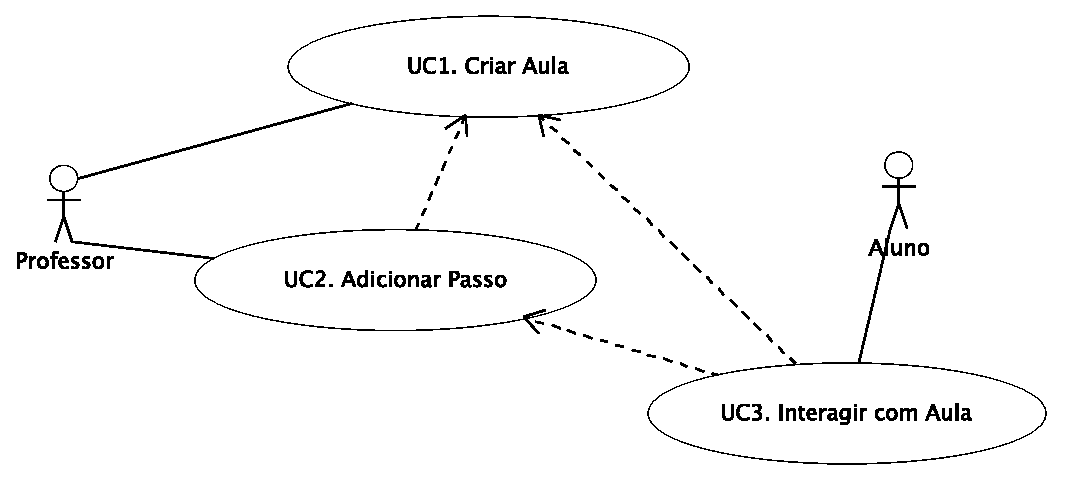
\includegraphics[scale=0.65]{../trabalho_full/casos.eps}
	\end{center}
\end{frame}

\begin{frame}{Diagramas de Classe}
	\begin{center}
		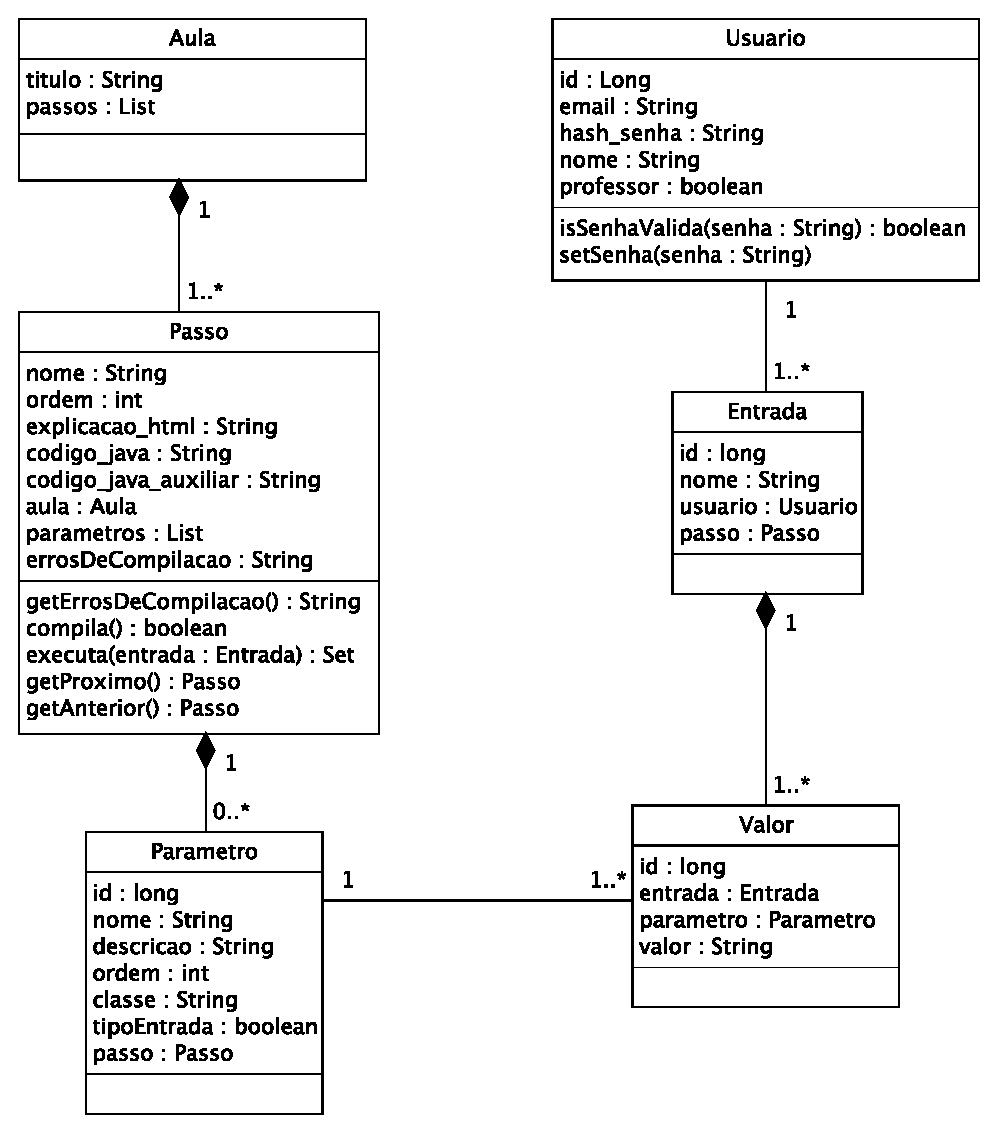
\includegraphics[scale=0.4]{../trabalho_full/classes.eps}
	\end{center}
\end{frame}

\section{Arquitetura de Software}

\begin{frame}{Escolha da Linguagem}
	Cada uma apresenta suas vantagens:
	\begin{itemize}
		\item C/C++: Performance
		\item Pascal: Simplicidade
		\item Fortran: Material Acadêmico
		\item Java: Equilíbrio destes fatores; facilidade para compilação dinâmica; JAMA
	\end{itemize}
\end{frame}

\begin{frame}{Padrões de Projeto}
	\begin{itemize}
		\item Mapeamento Objeto-Relacional
		\item Model / View / Controller
		\item Inversão de Controle / Injeção de Dependências
	\end{itemize}
\end{frame}

\begin{frame}{Componentes}
\begin{center}
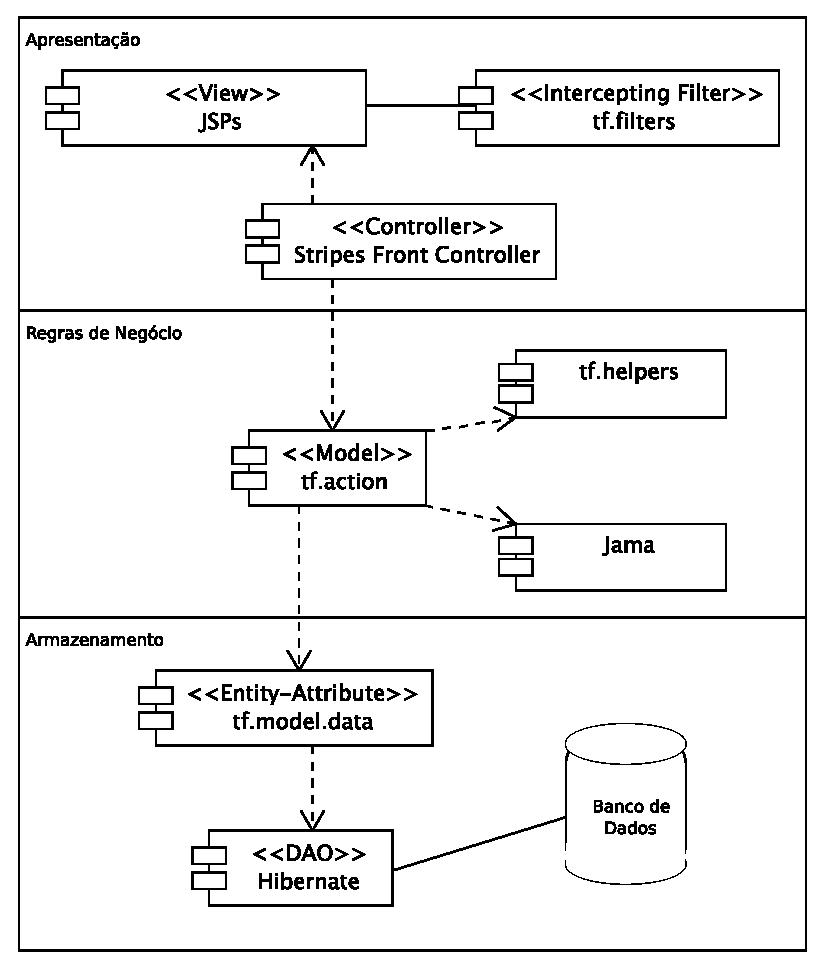
\includegraphics[scale=0.4]{../trabalho_full/deployment.eps}
\end{center}
\end{frame}


\begin{frame}{Compilação Dinâmica de Algoritmos}
	\begin{itemize}
		\item Idéia: usar a própria linguagem para executar os algoritmos
		\item Cadastro do Algoritmo (ex.: Cálculo de Juros):
		\begin{itemize}
			\item Parâmetros de Entrada\\\textit{(taxa, valor)}
			\item Parâmetros de Saída \\\textit{(juros)}
			\item Algoritmo \\\textit{(juros = valor*taxa; valor = valor + juros)}
			\item Código Auxiliar (opcional)\\ \textit{(função para Tabela Price)}
		\end{itemize}
		\item O sistema monta o código em tempo real usando estes elementos, e o \textit{javac} se encarregad o resto.
	\end{itemize}
\end{frame}

\begin{frame}
\begin{center}
\structure{\Huge Demonstração}
\end{center}
\end{frame}

\section{Uma Aula Prática}

\begin{frame}{Um Problema Econométrico (retomando)}
Modelo:
\[ y_t = \theta_1 + \theta_2 x_{t2} + (\theta_2)^2 x_{t3} +e_t , t = 1,2,...,20 \]
\[ y = f(\theta)+e\]
Função-Objetivo: \[H(\theta) = [y - f(\theta)]'[y - f(\theta)] \]
\end{frame}

\begin{frame}{Métodos de Gradiente}
\begin{block}{Idéia Geral}
$ \theta_{n+1} = \theta_{n} - t_{n}P_{n}\gamma_{n} $

\begin{itemize}
\item $P_{n}$: direção
\item $t_{n}$: "distância"
\item $\gamma_{n}$: gradiente de H
\end{itemize}
\end{block}
\begin{block}{Condições de Parada}
\begin{enumerate}
\item $ ( \theta_{n+l} - \theta_n )'( \theta_{n+l} - \theta_n ) < \epsilon$
\item $ H(  \theta_n )- H (\theta_{n+l} ) < \epsilon$
\item $  [\frac{\partial H}{\partial \theta}\vert_{\theta_n}]'[\frac{\partial H}{\partial \theta}\vert_{\theta_n}] < \epsilon$
\end{enumerate}
\end{block}

\end{frame}

\begin{frame}{Newton-Rhapson}
Usar o inverso da matriz Hessiana para especificar a direção do passo em cada iteração, ajustando-o pelo gradiente, isto é:
\[ \theta_{n+1} = \theta_{n} - \mathcal{H}_{n}^{-1}\gamma_{n}  \]


$\mathcal{H}_n$: Hessiano de $H(\theta)$ aplicado em $\theta_n$, isto é:

\[  \mathcal{H}_n = \left [ \left . \frac{\partial^2 H}{\partial \theta \partial \theta'} \right |_{\theta_n}  \right ] \]

\end{frame}

\begin{frame}{Newton-Rhapson: implementando}
\small{\texttt{double[][] hess = hess(theta1, theta2, y, x2, x3);\\
Matrix invHess = new Matrix(hess).inverse();\\
Matrix grad = new Matrix(\\\hspace{2pc}gradH(theta1, theta2, y, x2, x3), 2);\\
Matrix passo = invHess.times(grad);}}
\end{frame}


\begin{frame}{Gauss-Newton}


Definindo $ Z(\theta)=[\partial f/ \partial \theta'\vert_{\theta}] $, o passo é dado por:

\[ \theta_{n+1} = \theta_{n} + [Z(\theta_n)'Z(\theta_n)]^{-1}Z(\theta_n)'[y-f(\theta_n)] \]

que é o EMQ para o modelo:
\[ \bar{y}(\theta_n)=Z(\theta_n)\theta+e \]

\begin{block}{Caracterísitcas}
\begin{itemize}
	\item{Funciona como uma sequência de regressões lineares}
	\item{Restrito a funções-objetivo que são somas de quadrados
		\\\textit{ótimo: $ H(\theta) = [y - f(\theta)]'[y - f(\theta)] = e(\theta)'e(\theta) $}}
\end{itemize}
\end{block}
		
\end{frame}

\begin{frame}{Gauss-Newton: implementando}
\small{\texttt{Matrix Z = Z(theta1, theta2, x2, x3); \\
Matrix Zt = Z.transpose(); \\
Matrix f = f(theta1, theta2, x2, x3); \\
Matrix passo = Zt.times(Z).inverse()\\\hspace{2pc}.times(Zt)\\\hspace{2pc}.times(y.minus(f)).times(-1); }}
\end{frame}

\begin{frame}
\begin{center}
\structure{\Huge Demonstração}
\end{center}
\end{frame}

\section{Conclusão}

\begin{frame}{Lições Aprendidas}
	\begin{itemize}
		\item Não subestimar o aspecto educacional/didático
		\item É difícil conciliar simplificação e funcionalidades - mas coompensa
	\end{itemize}
\end{frame}

\begin{frame}{Sugestões para Continuidade}
	\begin{itemize}
		\item Cadastro de usuários (possivelmente vinculado a algum sistema de matrícula);
		\item Possibilidade de salvar e recuperar dados;
		\item Permitir ao código decidir o próximo passo a ser executado;
		\item Uma interface mais amigável para o professor (em particular na visualização do texto das aulas e da depuração do código dos algoritmos);
		\item Possibilidade de usar outros sistemas de codificação, como \LaTeX  /MathML na composição da parte teórica;
		\item Conversão semi-automática de algoritmos em outras linguagens (ex.: FORTRAN).
	\end{itemize}
\end{frame}

\begin{frame}
\begin{center}
\structure{\Huge Obrigado!}
\end{center}
\end{frame}








\end{document}


